\documentclass[a4paper, 12pt]{article}
\usepackage{lmodern}			% Usa a fonte Latin Modern
\usepackage[T1]{fontenc}		% seleção de códigos de fonte.
\usepackage[utf8]{inputenc}		% determina a codificação utiizada (conversão automática dos acentos)
\usepackage{hyperref}  			% controla a formação do índice
\usepackage{parskip}			% espaçamento entre os parágrafos
%\usepackage{microtype} 			% para melhorias de justificação
\usepackage{morefloats}			% permite mais floats
\usepackage{indentfirst}
\usepackage{graphicx}
\usepackage{float}
\usepackage[table]{xcolor}

\setlength{\parindent}{5ex}

% Babel e ajustes
\usepackage[british,UKenglish,USenglish,english,american]{babel}		% idiomas
\usepackage{listings}

\usepackage{color}
\definecolor{thered}{rgb}{0.65,0.04,0.07}
\definecolor{thegreen}{rgb}{0.06,0.44,0.08}
\definecolor{thegrey}{gray}{0.5}
\definecolor{theshade}{rgb}{1,1,0.97}
\definecolor{theframe}{gray}{0.6}
\definecolor{blue}{RGB}{41,5,195}


\pagestyle{plain}
\title {
			{\LARGE{\textbf{UNIVERSITY OF SOUTH WALES}}}\\
			{\large{\textsf{Faculty of Computing, Engineering and Science}}}\\
			{\large{\textsf{Computing Individual Project}}}\\
			\vspace{2.0cm}
			{\LARGE{\textbf{Automate Manual Task for Penetration Testing}}}
			\vspace{2.0cm}
}
\author { Brenno Candido, 13205978 } % end author

%------------------------------------------------------------------------- 
% inicio do documento
\begin{document}
\maketitle \clearpage
\pagenumbering{roman}

\section*{Statement of Originality}
\addcontentsline{toc}{section}{Statement of Originality}

\clearpage

\section*{Abstract}
\addcontentsline{toc}{section}{Abstract}

	Penetration Testers usually have to make their own scripts when they are testing a determined system or service. The proposal of this project is to
create a simple management console tool to speedup time during the manual process of a Penetration Test. This console application will be able to run a
collection of predefined scripts, other console tool, and predefined commands in a modular (plug-in) manner. The main characteristics of the project
are: easily adaptable and expandable due to a number of possible types of heterogeneous tests. The current project is focused on researching and
creating a Simple Mail Transfer Protocol Plugin (SMTP Plugin).\\

\clearpage

\section*{Acknowledgements}
\addcontentsline{toc}{section}{Acknowledgements}

\clearpage

\tableofcontents \clearpage
\pagenumbering{arabic}

\section{Introduction and Objectives}

\section{Research undertaken}

In the beginning, a research was made to gain background information about the topics that are potentially important to achieve the main objects of this project i.e. create a expandable and generic console tool application in order to automate manual tasks to speedup test and checks during a Penetration Testing Process. The research was based on finding related works and technologies used in the development process of the tool. Furthermore, to create a SMTP Plugin tool, a research about the main characteristics of smtp protocol, smtp servers, how to check they and, where Pen Testers can potentially explore in order to attack or gathering information.

\subsection{Related Works}

In order to provide a better understand about what to achieve to develop a expandable and generic console tool application, this session will focus on others tools that are related to this work. Firstly, a network infrastructure tool designed to automate and speed up the penetration testing process. Secondly, a tool made to perform tests to SMTP Server. Both tools has similarities and differences that will be highlighted in their section.


\subsubsection{Sparta - Network Infrastructure Penetration Testing Tool}

Sparta is a python GUI application which has almost the same goal as this project: an application to save time during some stage of the Penetration Test. Sparta was made to help penetration testing against network infrastructure. It can be used at the scanning and enumeration stage (Sparta Secforce, 2015). Sparta also helps tester save time by having point-and-click access to the tester's toolkit and by displaying the outputs in a nice and convenient way. However, Sparta does not do everything automatically, the tester has to take a time to set up the commands application needs to run. It is another point of similarity with this project, both  have a time consumption for the tester setting up the commands that will be performed. Sparta gives to the tester more time to focus on analysing the results instead of waste time performing the tests manually command-by-command. 

\subsubsection{NetScanTool}

In order to provide another example of a related work. This next tool that will be shown is a good example of a test/check SMTP Server, which are one important goal of the project. This tool is called NetScanTool. Its is designed  to be a SMTP Server Test Tool providing tests by sending email message through an SMTP Server. Its also allow to access and edit email header parameters such as From, To, Date, and Subject. NetScanTool provides supports to SMTP Authentication, basic or using STARTTLS with username and password. As another extended feature of this tool is the Email Relay Testing tool that comes with 17 common relay tests by communicating with a SMTP server. Even NetScanTool has a good set of testing tool, however its does not provide an extensibility to add different tests or customize predefined tests.

\subsection{Simple Mail Transfer Protocol}

Simple Mail Transfer Protocol are the most mail exchange used over the internet. This is an Internet standard that uses by default Transmission Control Protocol (TCP) on port 25, and for secure connection known as SMTPS uses TCP on port 465, however SMTPS on port 465 is not a standard even being widely used. A SMTP Server listen for connection, whereas a SMTP Client has to attempt to connect to the server. SMTP Servers respond with a three digit code, where the first digit indicates success or failure, and the next two digits provide more specific details about the response message, for further informations about SMTP Response codes check RFC 3463 (2003). After a connection being accepted and established by the server, the client at this point can interact with the server, and send an email.

\subsubsection{Sending Mail via Telnet}

In order to demonstrate a simple usage of SMTP Protocol, this section will show step by step of how to send an email using Telnet, the simplest TCP/IP command-line oriented tool (Korra'ti, 2005). By using a command line tool, and having a Telnet setup in the machine. Firstly, a connection will be created between the machine and a the SMTP Server on a certain port. It can be done by running the following command:

telnet [smtp-server] [port]
telnet mail.port25.com 25

If the connection succeed, a response that looks like this:

\noindent
\begin{figure}
	\centering
	\includegraphics[width=\textwidth]{images/sendmail_01.png}
	\caption{Send Mail}
	\label{img:sendmail_01}
\end{figure}

\noindent
notice the response code was 220, that means that the connection succeeded, however the server could respond with a 5.x.x response message if the server is unavailable in that moment for some reason causing a failure in the connection. Now, the connection was created and the SMTP Server waits for requests of the client. The client needs to specify a domain to talk to by typing:

EHLO [domain] or HELO [domain]
EHLO mx1.emailsrvr.com

A similar response will be display:
\begin{figure}
	\centering
	\includegraphics[width=\textwidth]{images/sendmail_02.png}
	\caption{Send Mail}
	\label{img:sendmail_02}
\end{figure}

Now, to continue sending an email, the client needs specify sender and receiver:

MAIL FROM: <sender email address>
RCPT TO: <receiver email address>

\begin{figure}
	\centering
	\includegraphics[width=\textwidth]{images/sendmail_03.png}
	\caption{Send Mail}
	\label{img:sendmail_03}
\end{figure}

Once all addresses have been specified, to write the email content type DATA, and then write the email content. After finish to type the email content, type a single dot in a new line. The server now will respond if the email request was accepted or not. To leave the connection type QUIT and the connection will be closed. This process can be seen in the nexts images

\begin{figure}
	\centering
	\includegraphics[width=\textwidth]{images/sendmail_04.png}
	\caption{Send Mail}
	\label{img:sendmail_04}
\end{figure}

\begin{figure}
	\centering
	\includegraphics[width=\textwidth]{images/sendmail_05.png}
	\caption{Send Mail}
	\label{img:sendmail_05}
\end{figure}

\subsection{SMTP Server Tests and Checks}

\section{Implementation}

	To reach the goals of this project, a python script called Taskrunner was developed as well as a xml structure was defined to be interpreted by the
Taskrunner. This xml structure is called a descriptor file. It basically contains a number of tasks/checks desired to be executed by the script. The
following session will discuss the main parts of the tool implemented i.e descriptor file and the script file. Firstly, what is the description file,
how to interpret it and how to expand it. Secondly this report will explain the usage of the Taskrunner, how it works, and how the script will interact
with the descriptor file.\\

\subsection{Descriptor File}

	The descriptor file was created to provide good usage and easy extensibility. This file contains plugins to be executed, and each plugin is composed by
tasks, descriptions and commands. In order to achieve a better understand of the descriptor architecture, this section will explain the structure
hierarchy and the element compositions.\\

	The structure hierarchy is composed by a combination of elements. The main elements used are: plugin, task and command, and their composition are
explained below:

\begin{itemize}
\item Each plugin has a plugin name, plugin description and a list of task;
\item Each task has a description and one or more commands to be executed; and
\item A command is defined by a shell command, a predefined script or other console tools
\end{itemize}

\noindent
The structure of the descriptor file can be seen in the Figure ~\ref{img:diagram}.

\noindent
\begin{figure}
	\centering
	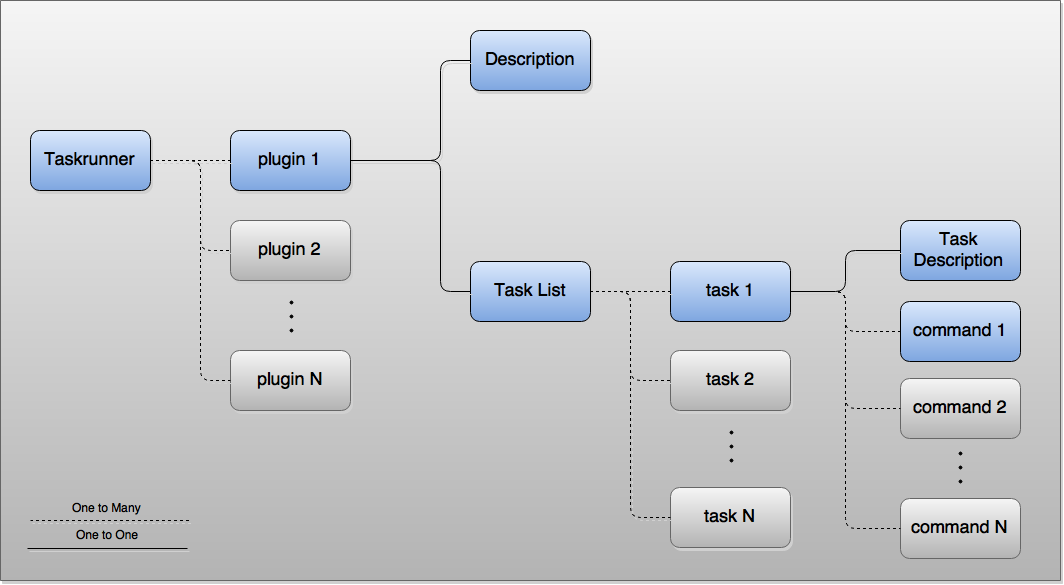
\includegraphics[width=\textwidth]{images/diagram.png}
	\caption{Descriptor Structure}
	\label{img:diagram}
\end{figure}

	Extensible Markup Language also known as XML provides a nice and clean way to describe the structure of the descriptor file. Although there are other
possibles formats that fits this structure like JSON or other text-based format, XML is easy to read and understand, and it make easier for expand the
functionalities such as add task/checks against HTTP Server, Web Servers, DNS Servers. This project will also provide a SMTP Plugin that will task/check
against SMTP Servers. More information is available in the SMTP Plugin session.\\

\subsection{Expand the Descriptor File}

	One of the biggest advantages of implementing the descriptor file in XML is due to the fact that XML provides a flexible structure to add and modify
data. This facility allows Pen Testers to add and modify/check tasks in a simple way. For example, if the Pen Tester wants to add different tasks or
add a new plugin to perform a range of different attacks against a Web server, an HTTP Server. The Pen Tester can also create a plugin that perform an
only checkup to gain time during the penetration test. In order to achieve this asset, a simple XML file is shown below to provide a basic view of the
Descriptor structure.\\

\clearpage

\lstset{
	language=xml,
	tabsize=3,
	float,
	%frame=lines,
	caption=	,
	label=code:sample,
	frame=shadowbox,
	rulesepcolor=\color{gray},
	xleftmargin=20pt,
	framexleftmargin=15pt,
	keywordstyle=\color{blue}\bf,
	commentstyle=\color{OliveGreen},
	stringstyle=\color{red},
	numbers=left,
	numberstyle=\tiny,
	numbersep=5pt,
	breaklines=true,
	showstringspaces=false,
	basicstyle=\footnotesize,
	emph={food,name,price},emphstyle={\color{magenta}}
}
\lstinputlisting{xmls/01_xml.xml}

	All Tasks has one or more shell commands to be executed, and it is nice to add a description of each task. It is recommended because Taskrunner provides
a list of task descriptions, and this feature improves the task visualization. Plugins are composed by a list of tasks and a plugin description. The
description is optional, however it is recommended to add as well as it is recommended for task descriptions. Therefore, to add a new task in a plugin,
a task tag should be added inside the taskList tag, and the new task tag should be composed by a description and a command.\\

	In almost the same way that tasks are added, it is possible to expand the Descriptor to contain many plugins by adding new plugins. To add a new plugin,
a plugin tag should be added inside the taskrunner tag. The new plugin tag should contain a plugin description and a task list. A taskList tag is
composed by many tasks tag.\\

\subsection{Taskrunner}

	Taskrunner is a python script developed to interpret and execute the tasks specified in the Descriptor file. Python was chosen due to the fact that is
easy and simple. Python also provides a fast development, and it is easy to read and to understand. Furthermore, python comes with many useful built-in
tools like XML Parsers and String methods, which makes the development easier and faster than programming in a language without these built-methods,
such as C Language. Taskrunner provides a command line interaction with console tools such as Terminal and Command Prompt. This section will focus on
how make Taskrunner execute the plugins/tasks specified in described in the Descriptor file.\\

	Taskrunner should be executed via a command line. In order to execute the script make sure that Taskrunner has permission to execute. To execute,
a Descriptor file and a Plugin must be informed with option -D and option -P, respectively. In the example below, myDescriptor.xml is the Descriptor
file’s name, and myPlugin is the Plugin’s name. It is important to notice that all plugins must have a name. \\

	Taskrunner comes with functionalities to improve user experience and time performance. The pĺugin can also provide a description list of each task
on the Descriptor file using option --list. It can be very useful for descriptor files which many people might have access, and when plugin/tasks are
constantly modified. By default all the tasks are executed sequentially, and it can lead to bottleneck, since tasks are not linked to each other, for
example a considerable number of task can take a time to finish. Therefore, to increase the time performance, the tasks can be executed in parallel
using the option --parallel. Be aware that the --parallel option only parallelize tasks i.e. the commands inside a task is executed sequentially.\\

\noindent
Command-line executions:
\begin{lstlisting}
$ ./taskrunner.py -D myDescriptor.xml -P myPlugin
$ ./taskrunner.py -D myDescriptor.xml -P myPlugin  --list
$ ./taskrunner.py -D myDescriptor.xml -P myPlugin  --parallel
\end{lstlisting}

\noindent
Descriptor:
\begin{lstlisting}[language=xml]
<taskrunner>
  <plugin name="myPlugin"> ... </plugin>
</taskrunner>
\end{lstlisting}


\subsection{Variable}

	Commands-line arguments such as IP addresses and Port numbers are used many time in some stage a penetration test. Those types of command-line
arguments is an example of possible variable. In order to create reusable plugins in differents projects, the variable concept was introduced in the
Descriptor file. Variables are a simple string substitution that allow the user pass values through command line.\\

	Variables are defined into the command tag in the Descriptor file, and they are declared with predefined structure. The variable declaration in the
Descriptor file is composed by two parts: a variable marker followed by a variable name. Firstly, a variable marker is the percent sign (\%). The variable
name could be any string of numbers or/and characters. Therefore, to actually use the variable at the time to execute the script a option with the
variable name has to be passed as a command-line argument. To demonstrate a variable usage see the next example.\\

\noindent
Command-line executions:
\begin{lstlisting}
$ ./taskrunner.py -D myDescriptor.xml -P myPlugin -PATH /etc
$ ./taskrunner.py -D myDescriptor.xml -P myPlugin -ip 192.168.1.1
$ ./taskrunner.py -D myDescriptor.xml -P myPlugin -PATH /etc -ip 192.168.1.1 
\end{lstlisting}

\noindent
Descriptor:
\begin{lstlisting}[language=xml]
<command> ls %PATH </command>
<command> nmap %ip </command>
\end{lstlisting}

\subsection{SMTP Plugin}

\section{Results}

\section{Evaluation}

\section{Conclusion}



\newpage

\section*{References}

\end{document}